%
%	Sketches for Q2

%
%	Set A
%
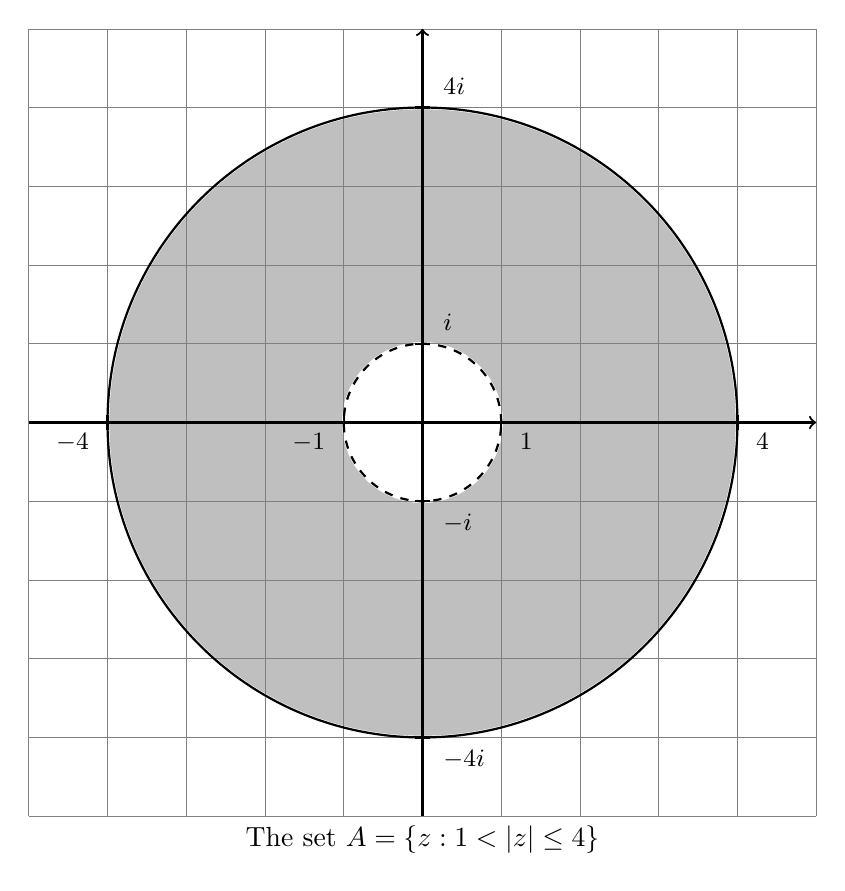
\begin{tikzpicture}
	% shading - must be drawn before the rest!
	\filldraw[even odd rule,color=lightgray] (0,0) circle(3.97) (0,0) circle(1.03);
	% grid for draft only
	\draw [help lines] (-5,-5) grid (5,5);
	% legend
	\draw (0,-5) node[below] {The set $A=\{z:1<|z|\le4\}$};
	% the X-axis
	\draw[->,thick] (-5,0)--(5,0);
	\draw[thick] (-4,-0.1) -- (-4,0.1) node[below left=3pt] {\small $-4$};
	\draw[thick] (-1,-0.1) -- (-1,0.1) node[below left=3pt] {\small $-1$};
	\draw[thick] (1,-0.1) -- (1,0.1) node[below right=3pt] {\small $1$};
	\draw[thick] (4,-0.1) -- (4,0.1) node[below right=3pt] {\small $4$};
	% the Y-axis
	\draw[->,thick] (0,-5)--(0,5);
	\draw[thick] (-0.1,-4) -- (0.1,-4) node[below right=1pt] {\small $-4i$};
	\draw[thick] (-0.1,-1) -- (0.1,-1) node[below right=1pt] {\small $-i$};
	\draw[thick] (-0.1,1) -- (0.1,1) node[above right=1pt] {\small $i$};
	\draw[thick] (-0.1,4) -- (0.1,4) node[above right=1pt] {\small $4i$};
	% inner circle border
	\draw[thick,style=dashed] (0,0) circle (1);
	% outer circle border
	\draw[thick] (0,0) circle (4);
\end{tikzpicture}

\bigskip

%
%	Set B
%
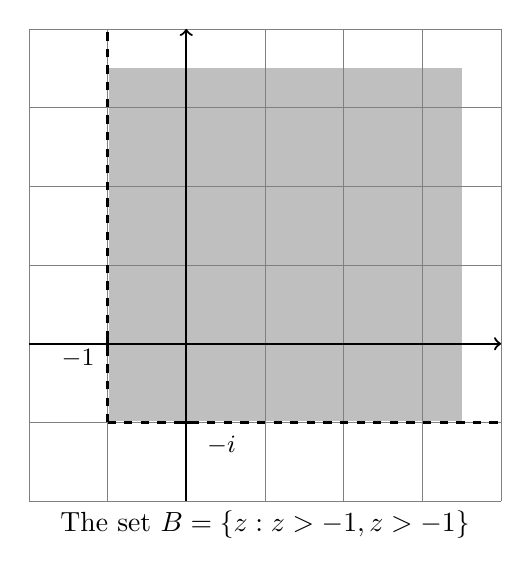
\begin{tikzpicture}
	% shading - must be drawn before the rest!
	\filldraw[color=lightgray] (-0.97,-0.97) -- (3.5,-0.97) -- (3.5,3.5) -- (-0.97,3.5) -- cycle;
	% grid for draft only
	\draw [help lines] (-2,-2) grid (4,4);
	% legend
	\draw (1,-2) node[below] {The set $B=\{z:\RE z>-1,\IM z>-1\}$};
	% the Y-axis
	\draw[->,thick] (0,-2)--(0,4);
	% the X-axis
	\draw[->,thick] (-2,0)--(4,0);
	\draw[thick] (-1,-0.1) -- (-1,0.1) node[below left=1pt] {\small $-1$};
	\draw[thick] (-0.1,-1) -- (0.1,-1) node[below right=1pt] {\small $-i$};
	% the two borders
	\draw[style=dashed,thick] (-1,-1) -- (4,-1);
	\draw[style=dashed,thick] (-1,-1) -- (-1,4);
\end{tikzpicture}

\bigskip

%
%	Set C
%
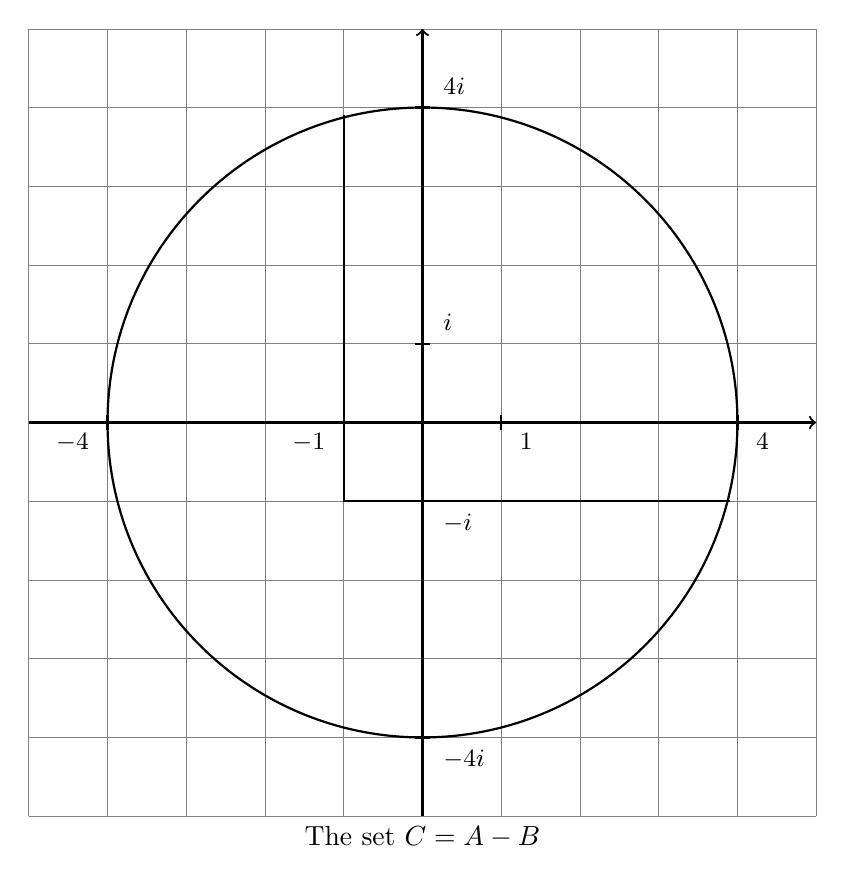
\begin{tikzpicture}
	% shading - must be drawn before the rest!
	%%\filldraw[even odd rule,color=lightgray] (0,0) circle(3.97) (0,0) circle(1.03);
	% grid for draft only
	\draw [help lines] (-5,-5) grid (5,5);
	% legend
	\draw (0,-5) node[below] {The set $C=A-B$};
	% the X-axis
	\draw[->,thick] (-5,0)--(5,0);
	\draw[thick] (-4,-0.1) -- (-4,0.1) node[below left=3pt] {\small $-4$};
	\draw[thick] (-1,-0.1) -- (-1,0.1) node[below left=3pt] {\small $-1$};
	\draw[thick] (1,-0.1) -- (1,0.1) node[below right=3pt] {\small $1$};
	\draw[thick] (4,-0.1) -- (4,0.1) node[below right=3pt] {\small $4$};
	% the Y-axis
	\draw[->,thick] (0,-5)--(0,5);
	\draw[thick] (-0.1,-4) -- (0.1,-4) node[below right=1pt] {\small $-4i$};
	\draw[thick] (-0.1,-1) -- (0.1,-1) node[below right=1pt] {\small $-i$};
	\draw[thick] (-0.1,1) -- (0.1,1) node[above right=1pt] {\small $i$};
	\draw[thick] (-0.1,4) -- (0.1,4) node[above right=1pt] {\small $4i$};
	% inner border
	\draw[thick] (-1,3.9) -- (-1,-1) -- (3.9,-1);
	% outer circle/arc
	\draw[thick] (0,0) circle (4);
\end{tikzpicture}

\bigskip

%
%	Set D
%
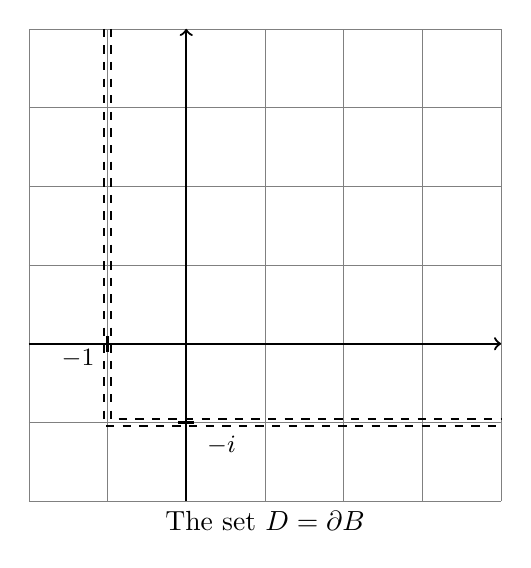
\begin{tikzpicture}
	% grid for draft only
	\draw [help lines] (-2,-2) grid (4,4);
	% legend
	\draw (1,-2) node[below] {The set $D=\partial B$};
	% the Y-axis
	\draw[->,thick] (0,-2)--(0,4);
	% the X-axis
	\draw[->,thick] (-2,0)--(4,0);
	\draw[thick] (-1,-0.1) -- (-1,0.1) node[below left=1pt] {\small $-1$};
	\draw[thick] (-0.1,-1) -- (0.1,-1) node[below right=1pt] {\small $-i$};
	% the empty border!
	% - outer side of the L
	\draw[thick,style=dashed] (-1.04,4) -- (-1.04,-1.04) -- (4,-1.04);
	% - inner side of the L
	\draw[thick,style=dashed] (-0.96,4) -- (-0.96,-0.96) -- (4,-0.96);
\end{tikzpicture}

